\section{Atomic Swap and American Call Option}
\label{sec:formalization}

In this section, we describe the Atomic Swap protocol (the original version on Bitcointalk~\cite{nolan2013alt}) and the American Call Option,
then point out that an Atomic Swap is equivalent to an American Call Option without the premium.





\subsection{Atomic Swap}

\subsubsection{Security assumptions}

We first give security assumptions on the Atomic Swap.

First, we assume blockchains involved in the Atomic Swap are secure, and execute all transactions correctly.
The Atomic Swap is based on blockchains.
If the blockchains are insecure, the Atomic Swap will also be insecure.

Second, we assume the HTLC mechanism in blockchains is reliable.
More specifically,
1) blockchains produce new blocks with stable speeds;
2) the hash algorithm used by HTLCs is secure;
3) the runtime for executing HTLCs is reliable.


Third, the time for confirming a transaction is negligible compared to timelocks.
In practice, the swap initiator's timelock is 48 hours and the swap participant's timelock is 24 hours by default~\cite{nolan2013alt}, while confirming a transaction is less than 1 hour for most blockchains.


\subsubsection{Process}


\begin{figure}
    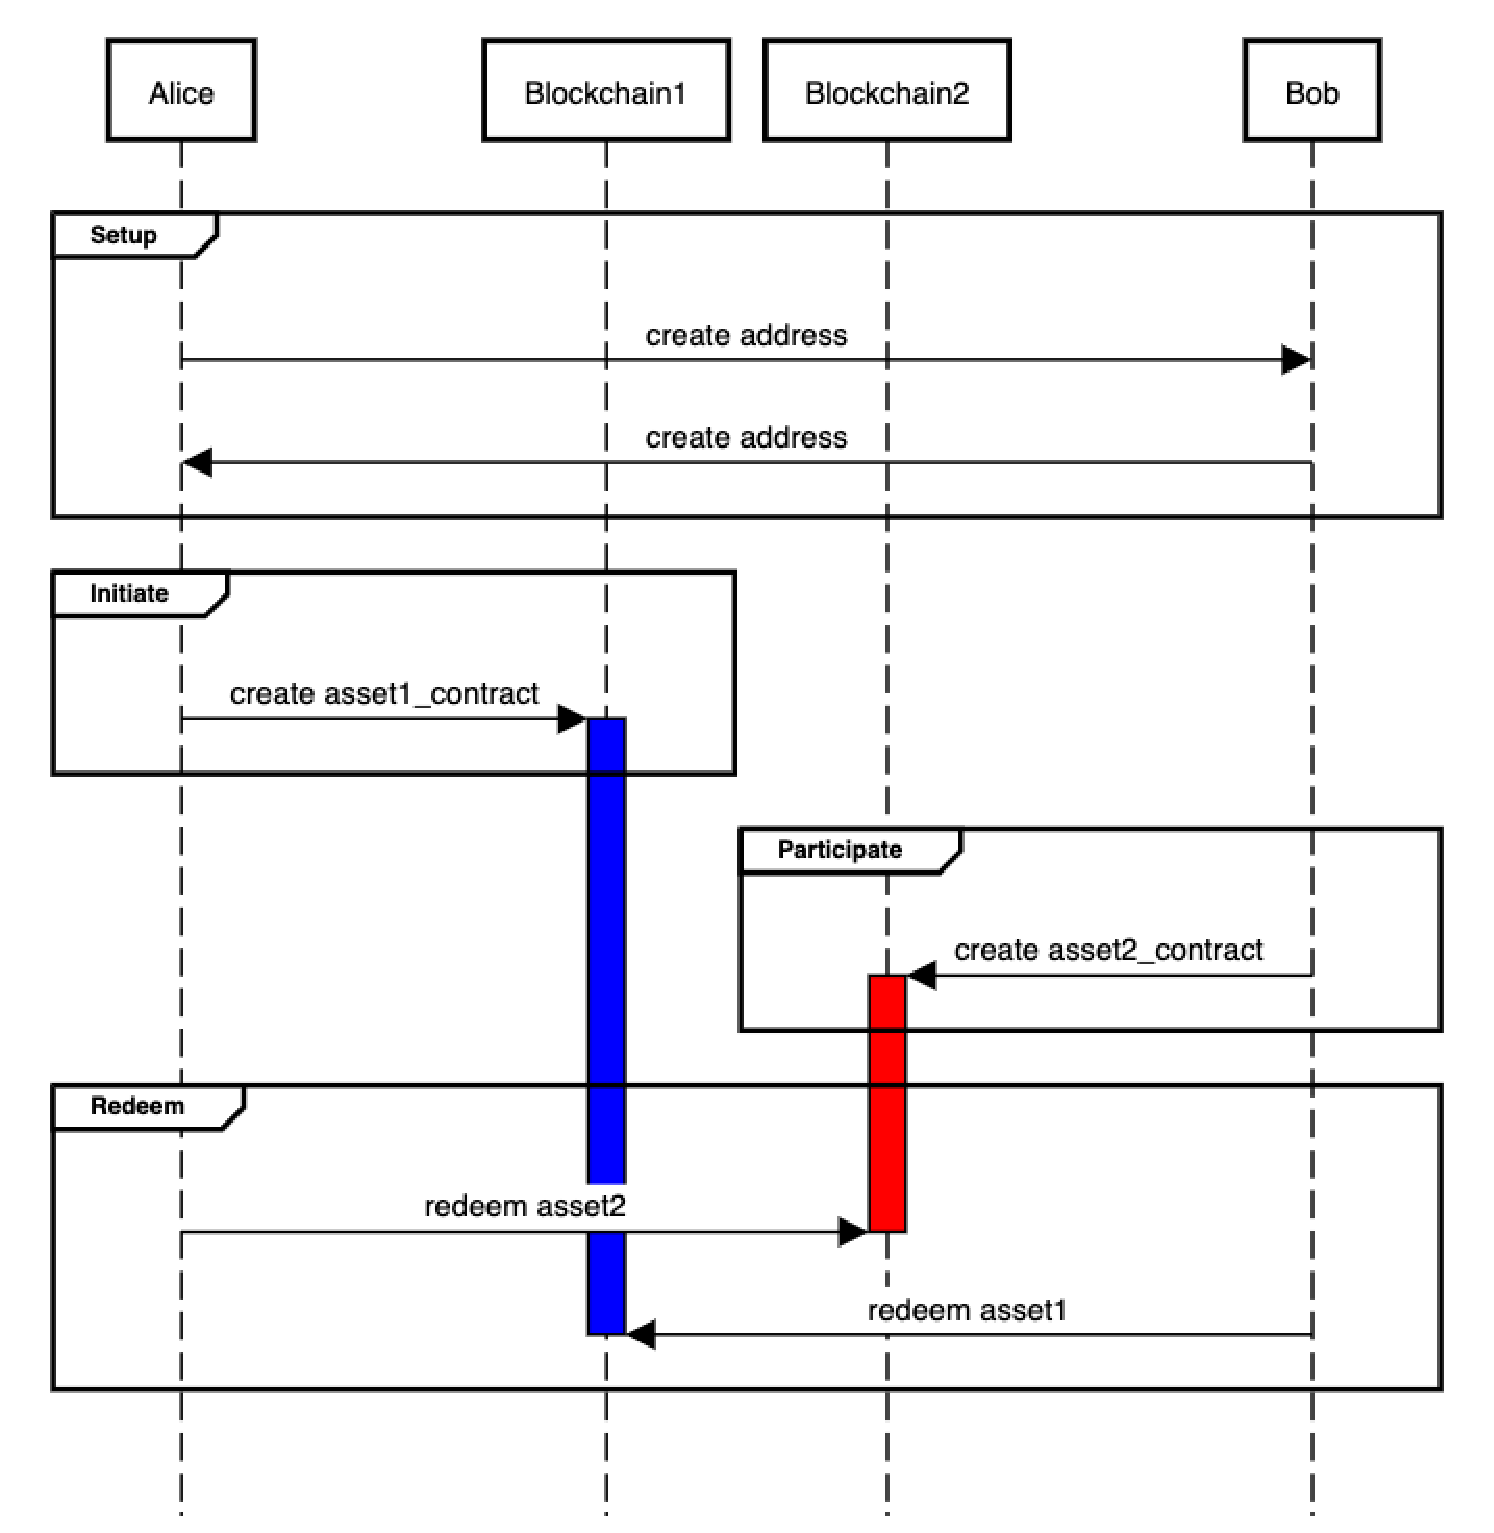
\includegraphics[width=.7\linewidth]{sequence_diagram_original.eps}
    \caption{Sequence diagram of the Atomic Swap.}
    \label{fig:sequence_diagram_original}
\end{figure}

\begin{figure}
    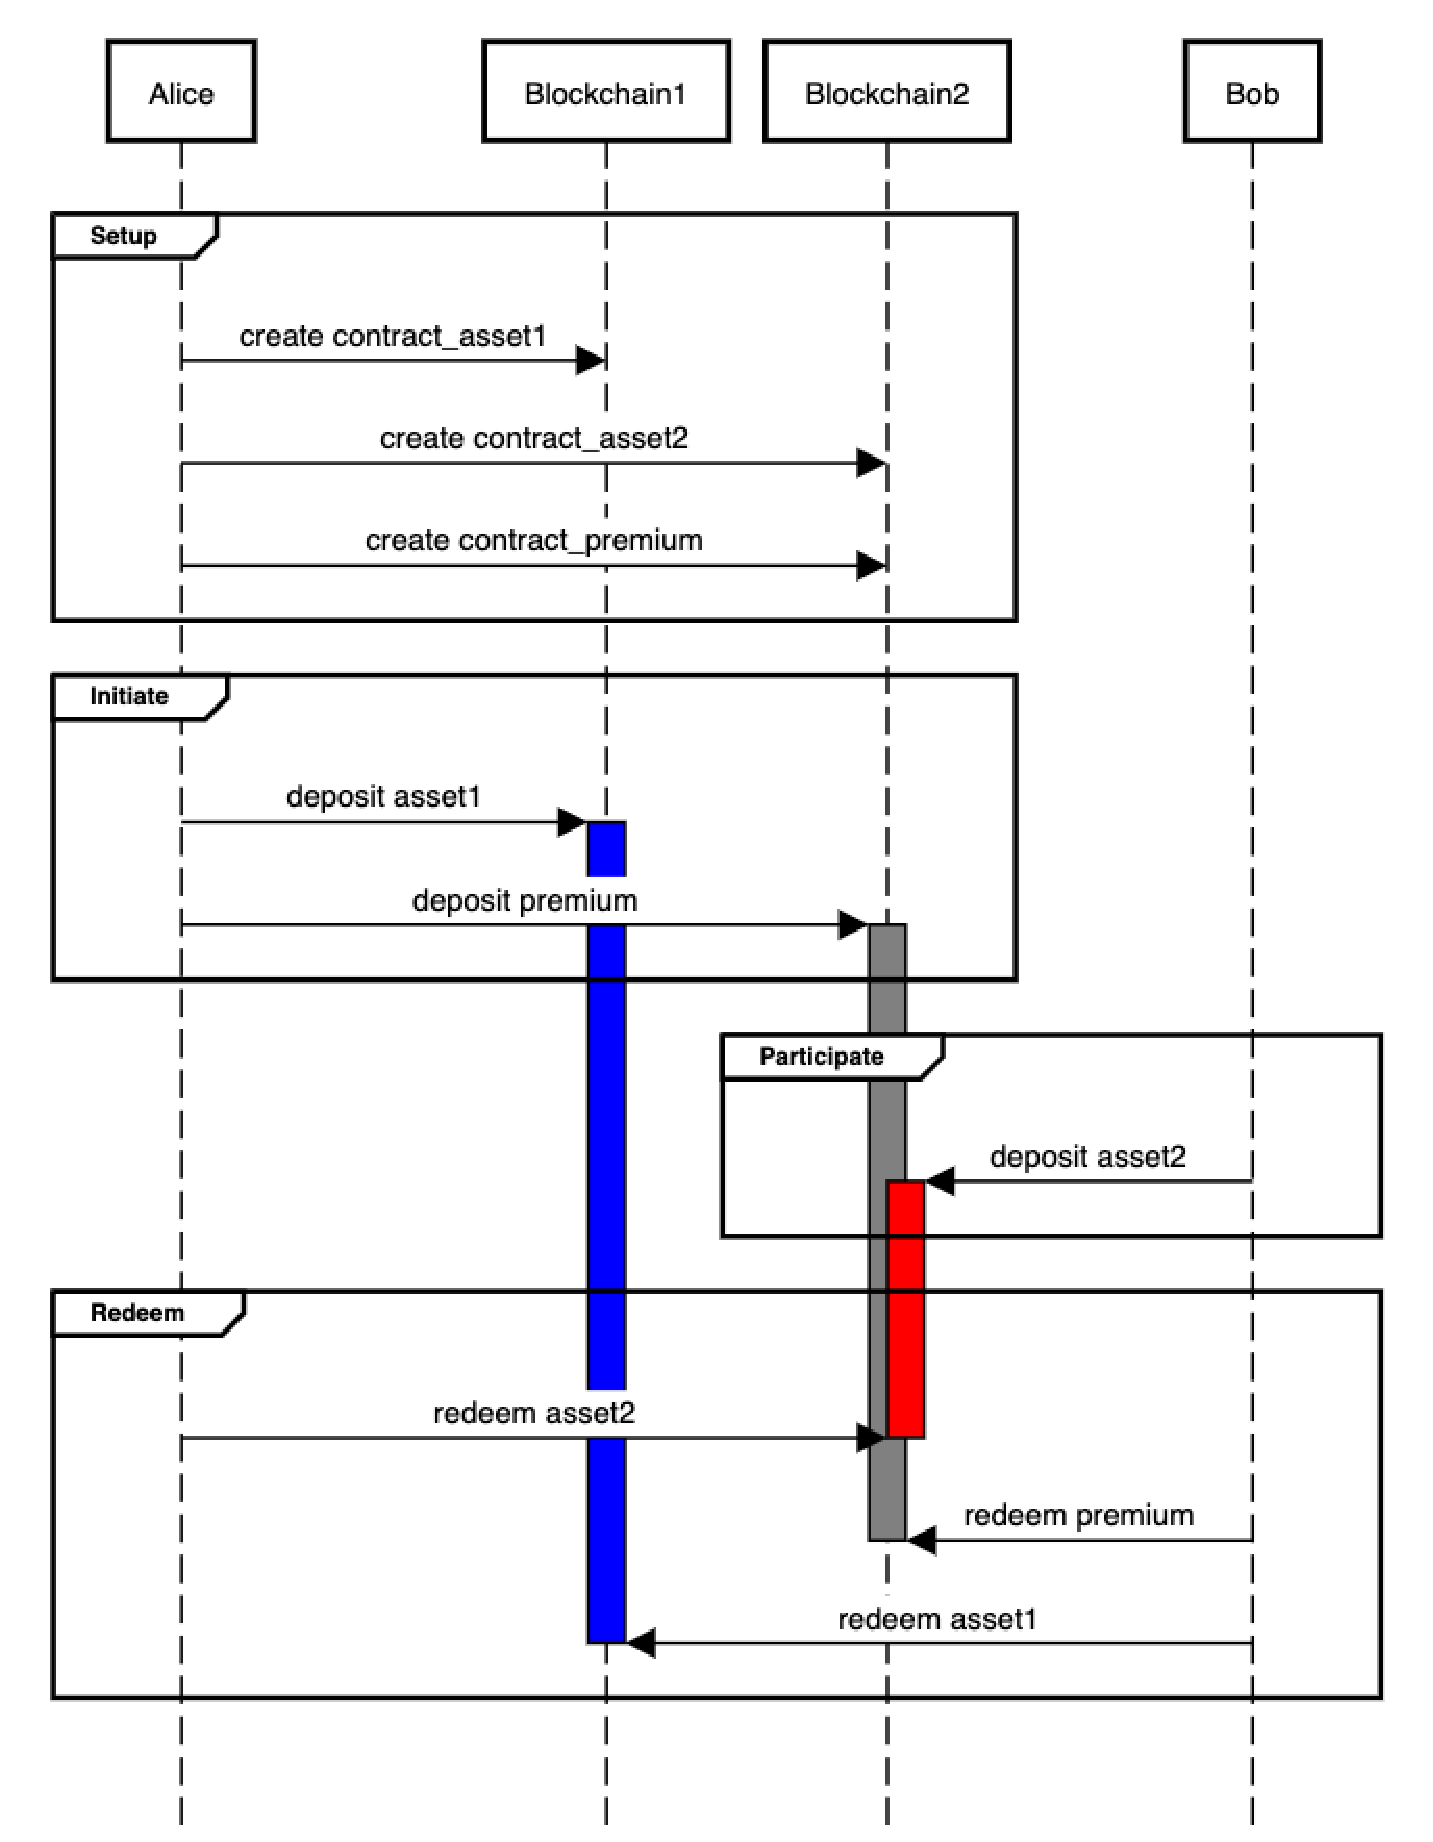
\includegraphics[width=.7\linewidth]{sequence_diagram_options.eps}
    \caption{Sequence diagram of the American Call Option.}
    \label{fig:sequence_diagram_option}
\end{figure}



Assume the swap initiator Alice hopes to get $x_2$ $Coin_2$ from the swap participant Bob in exchange of $x_1$ $Coin_1$. 
$Coin_1$ is the cryptocurrency on the blockchain $BC_1$, and $Coin_2$ is the cryptocurrency on the blockchain $BC_2$.

We denote the swap as $\mathcal{AS} = (x_1, Coin_1, x_2, Coin_2)$.
Let Alice be the holder of the address $\beta_{A, 1}$ on $BC_1$ and the address $\beta_{A, 2}$ on $BC_2$.
Let Bob be the holder of the address $\beta_{B, 1}$ on $BC_1$ and the address $\beta_{B, 2}$ on $BC_2$.
$\beta_{A, 1}$ holds $Coin_1$ with the amount more than $x_1$, and $\beta_{B, 2}$ holds $Coin_2$ with the amount more than $x_2$.

Figure~\ref{fig:sequence_diagram_original} shows the process of $\mathcal{AS}$.
More specifically, $\mathcal{AS}$ consists of five steps:
\textbf{Initiate},
\textbf{Participate},
\textbf{Redeem}, and
\textbf{Refund}.


\paragraph{\textbf{Initiate}}
Alice initiates $\mathcal{AS}$ at this stage.
% s and h
First, Alice picks a random secret $s$, and computes the hash $h = \mathcal{H}(s)$ of $s$, where $\mathcal{H}$ is a secure hash function.
At this stage, $s$ is only known to Alice.
% contract
Then, Alice creates the contract script $\mathcal{C}_1$ that ``Alice pays $x_1$ $Coin_1$ from $\beta_{A, 1}$ to $\beta_{B, 1}$ if Bob can provide $s$ which makes $\mathcal{H}(s) = h$ before or on a timelock $\delta_1$ (which is a timestamp). After $\delta_1$, Alice can refund the money - get $x_1$ $Coin_1$ back.''
% tx
After creating $\mathcal{C}_1$, Alice publishes $\mathcal{C}_1$ as a transaction $tx_{\mathcal{C}, 1}$ on $BC_1$.
Note that $h$ is published when publishing $tx_{\mathcal{C}, 1}$.
% refund
Besides $\mathcal{C}_1$, Alice also creates a refund script $\mathcal{R}_1$ that ``Alice pays $x_1$ $Coin_1$ from $\beta_{A, 1}$ to her another address.'' This is to ensure $x_1$ $Coin_1$ can no longer be redeemed by others. Alice can do this only after $\delta_1$.
If Bob does not redeem $x_1$ $Coin_1$ and $\delta_1$ expires, Alice can refund $x_1$ $Coin_1$ by publishing $\mathcal{R}_1$ as a transaction $tx_{\mathcal{R}, 1}$ on $BC_1$.

\paragraph{\textbf{Participate}}
Bob participates in $\mathcal{AS}$ at this stage after \textbf{Initiate}.
% contract
With the published $h$, Bob creates the contract script $\mathcal{C}_2$ that ``Bob pays $x_2$ $Coin_2$ from $\beta_{B, 2}$ to $\beta_{A, 2}$ if Alice can provide $s$ before or on a timelock $\delta_2$ (which is a timestamp). After the time of $\delta_2$, Bob can refund the money - get $x_2$ $Coin_2$ back.''
Here $\delta_2$ should expire earlier than $\delta_1$.
% tx
After creating $\mathcal{C}_2$, Bob publishes $\mathcal{C}_2$ as a transaction $tx_{\mathcal{C}, 2}$ on $BC_2$.
Note that Alice knows $s$ so she can redeem $x_2$ $Coin_2$ in $tx_{\mathcal{C}, 2}$ anytime before $\delta_2$.
% refund 
Besides $\mathcal{C}_2$, Bob also creates a refund script $\mathcal{R}_2$ that ``Bob pays $x_2$ $Coin_2$ from $\beta_{B, 2}$ to his another address.''
This is to ensure $x_2$ $Coin_2$ can no longer be redeemed by others. Bob can do this only after $\delta_2$.
If Alice does not redeem $x_2$ $Coin_2$ and $\delta_2$ expires, Bob can refund $x_2$ $Coin_2$ by publishing $\mathcal{R}_2$ as a transaction $tx_{\mathcal{R}, 2}$ on $BC_2$.

\paragraph{\textbf{Redeem} or \textbf{Refund}}

\textbf{Redeem.}
At this stage, Alice redeems $x_2$ $Coin_2$ by publishing $s$, then Bob can also redeem $x_1$ $Coin_1$ with the published $s$.
First, Alice provides $s$ to $tx_{\mathcal{C}, 2}$ in order to redeem $x_2$ $Coin_2$ in $tx_{\mathcal{C}, 2}$.
As a result, Alice redeems $x_2$ $Coin_2$, but exposes $s$ to Bob.
After that, Bob provides $s$ to $tx_{\mathcal{C}, 1}$ in order to redeem $x_1$ $Coin_1$ in $tx_{\mathcal{C}, 1}$.
In this way, Alice and Bob successfully exchanges $x_1$ $Coin_1$ and $x_2$ $Coin_2$.

\textbf{Refund.}
However, if Alice does not redeem $x_2$ $Coin_2$ after $\delta_2$ expires, Bob can refund his $x_2$ $Coin_2$ by publishing $tx_{\mathcal{R}, 2}$.
As a result, Alice cannot redeem $x_2$ $Coin_2$, and will not publish $s$.
After $\delta_1$, Alice can also refund her $x_1$ $Coin_1$ by publishing $tx_{\mathcal{R}, 1}$.


% why atomic
We can see that $\mathcal{AS}$ either succeeds or fails for both Alice and Bob.
In detail,

\begin{itemize}
    \item If Alice misbehaves when triggering \textbf{Initiate}, Bob will lose nothing as he hasn't deposited $x_2$ $Coin_2$ yet.
    \item If Bob misbehaves when triggering \textbf{Participate}, Alice can choose to abort $\mathcal{AS}$ by triggering \textbf{Refund}.
    \item Alice can only choose to redeem $x_2$ $Coin_2$ by triggering \textbf{Redeem} or wait $\delta_2$ to expire.
    Once Alice triggers \textbf{Redeem}, Bob can also trigger \textbf{Redeem}.
    Once $\delta_2$ expires, Bob can trigger \textbf{Refund} to get his $x_2$ $Coin_2$ back.
\end{itemize}

% misuse
However, one may take both $Coin_1$ and $Coin_2$ if the other does not trigger \textbf{Redeem} or \textbf{Refund} on time.
For example, if Bob does not trigger \textbf{Redeem} after Alice triggers \textbf{Redeem} and $\delta_1$ expires, Alice can also refund $x_1$ $Coin_1$ by triggering \textbf{Refund}.
But in this case it is Bob to blame, because he should have had enough time - at least $\delta_2 - \delta_1$ (48 - 24 = 24 hours by default) - to redeem $x_1$ $Coin_1$.
Another example is that Alice broadcasts $tx_{\mathcal{C}, 1}$ after $\delta_2$, but Bob has already triggered \textbf{Refund}.
Therefore, Bob can also trigger \textbf{Redeem} with the preimage in Alice's transaction of \textbf{Redeem} before $\delta_1$.
Similarly, it is Alice to blame, because she should have had enough time - before $\delta_2$ - to trigger \textbf{Redeem}.

Note that the exchange rate $Coin_2 / Coin_1$ is fluctuating overtime due to the market mechanism.
We denote the asset's underlying value (with the unit $\frac{Coin_2}{Coin_1}$) at the time $t$ as $S_t$.















\subsection{American Call Option}

The American Call Option is a contract that ``one can buy an amount of an asset with an agreed price prior to or on an agreed time in the future''. 
The agreed price is usually called the \textit{spot price}, and the buying is called \textit{exercising}.
For American Call Option, the option buyer can exercise in advanced of the agreed exercise time.
The price of the asset when exercising is called the \textit{strike price}.
As mentioned in Section~\ref{subsec:background_option}, the option contract itself has value, and its value is called the \textit{premium}.
The option buyer should pay for both the asset and the premium when participating in the contract.

More specifically, we denote an American Call Option contract $\Pi$ as

$$\Pi = (\pi_1, \pi_2, K, A, T, C)$$

where
$\pi_1$ and $\pi_2$ are the currency of the option buyer and the asset of the option seller, respectively; 
$K$ is the strike price with the unit $\pi_2 / \pi_1$ - the price of $\pi_2$ measured in $\pi_1$;
$A$ is the amount of the asset $\pi_2$ that the option seller wants to sell;
$T$ is the agreed strike time;
$C$ is the \textit{premium} with the unit $\pi_1$.

The process of an American Call Option is as follows:

\begin{enumerate}
    \item \textbf{Advertise}: The option seller creates and advertises an American Call Option contract $\Pi = (\pi_1, \pi_2, K, A, T, C)$.
    \item \textbf{Contract}: The option buyer finds $\Pi$ is profitable, so he participates in $\Pi$.
    To participate, the option buyer should pay $C$ to the option seller first.
    Note that the option buyer does not pay for $A$ $\pi_2$ at this stage.
    Also note that the option seller cannot abort $\Pi$ after the option buyer participates in $\Pi$.
    \item \textbf{Exercise} or \textbf{Abort}: The option buyer exercises $\Pi$ - pays $AK$ $\pi_1$ to the option seller - before or on $T$, and the option seller gives $A$ $\pi_2$ to the option buyer.
    If the option buyer does not exercise $\Pi$ before or on $T$, $\Pi$ will abort - the option buyer gets $\pi_1$ back and the option seller gets $\pi_2$ back and $C$. In other words, both of them get their underlying asset back, but the option buyer loses the premium $C$.
\end{enumerate}

% asset underlying value
Similar with the Atomic Swap, the exchange rate of $\pi_2 / \pi_1$ is also fluctuating overtime.
We denote the asset's underlying value (with the unit $\pi_2 / \pi_1$) at the time $t$ as $S_t$.












\subsection{An Atomic Swap is a premium-free American Call Option}

We show that an Atomic Swap is equivalent to a premium-free American Call Option.
More specifically, $\mathcal{AS} = (x_1, Coin_1, x_2, Coin_2)$ is equivalent to the American Call Option contract

$$
\Pi = (Coin_1, Coin_2, \frac{x_2}{x_1}, x_2, \delta_2, 0)
$$

where:
\textbf{Advertise} in the American Call Option is equivalent to \textbf{Initiate} in the Atomic Swap;
\textbf{Contract} in the American Call Option is equivalent to \textbf{Participate} in the Atomic Swap;
\textbf{Exercise} in the American Call Option is equivalent to \textbf{Redeem} in the Atomic Swap;
\textbf{Abort} in the American Call Option is equivalent to \textbf{Refund} in the Atomic Swap.


In the American Call Option context, the option buyer Alice wants to buy $x_2$ $Coin_2$ from the participant Bob by using $x_1$ $Coin_1$.
$Coin_1$ is the currency Alice uses, $Coin_2$ is the asset Bob has.
$\frac{x_2}{x_1}$ is the price of the asset from Alice's perspective, so $\frac{x_2}{x_1}$.
$\delta_2$ is the timelock of the contract transaction on $BC_2$.
It is equivalent to the strike time of $\Pi$, because after $\delta_2$ Bob can refund his asset back and invalidate $\mathcal{AS}$, but before $\delta_2$ Bob cannot abort $\mathcal{AS}$ if Alice triggers \textbf{Participate}.
Establishing the Atomic Swap does not require Alice to pay anything other than the asset to Bob, so the premium here is zero.